\section{Results and discussion} \label{isect4}

\subsection{Genderwise wage gap decomposition}

During the urban wage stagnation of the first decade, the highest male wage percentiles saw larger improvements in their position compared to women. Overall, above the median, the total gender gap deteriorated, whereas slight improvements were seen in the bottom quarter of the distribution (see figure \ref{fig:decomMainResultUrb}). In the lowest wage group ($\tau = 0.1$), the gap shrunk slightly, from -0.38 to -.35 units of log wage (see table \ref{tab:unadjDecom}). In the next decade, however, higher wage percentile ($\tau = 0.9$) improved their position drastically, overcoming the decline of 2008 and improving upon 1998's gender gap. However, the situation was less rosy for the rest: median women saw a slight slump in their position, and the lowest percentiles saw paltry improvements in view of both decades.\par 

\begin{figure}[bth] 
	\centering
	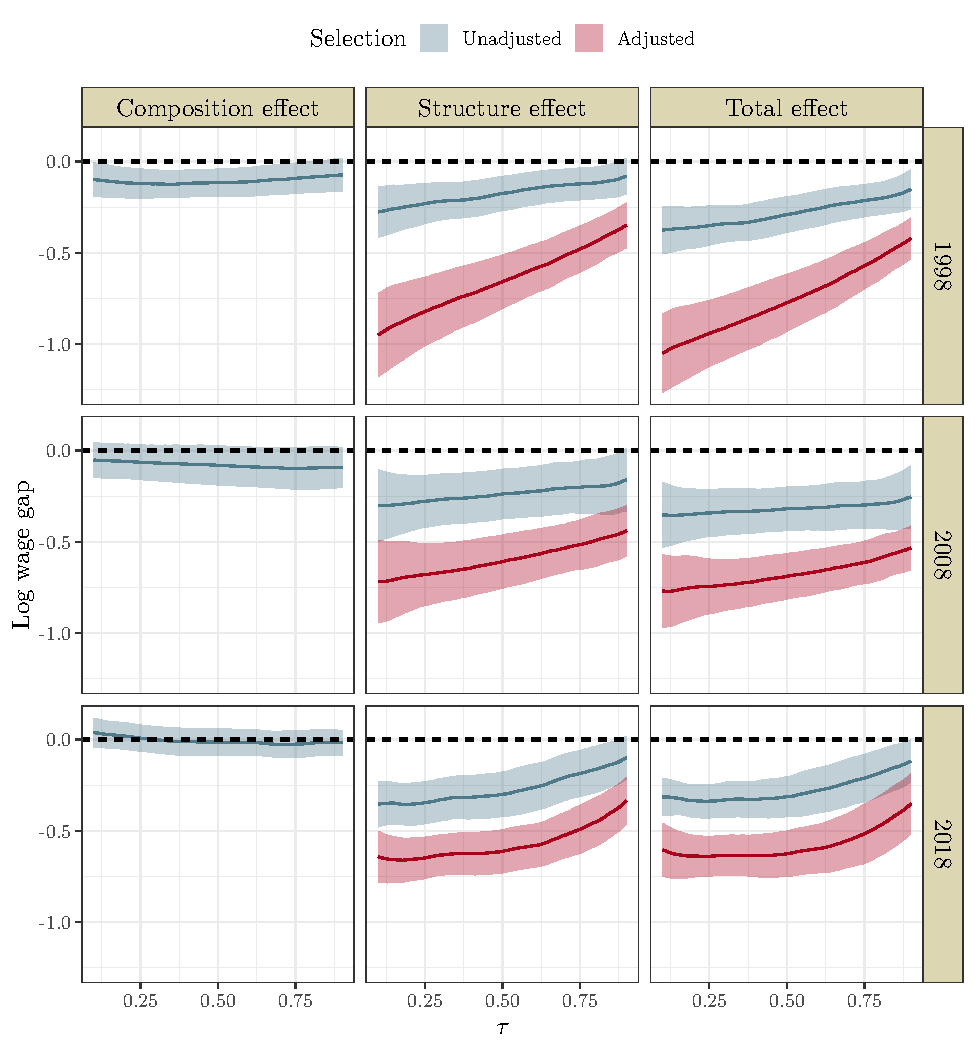
\includegraphics[width=.8\textwidth]{./figure/UrbanDecom_all_all}
	\caption{Urban wage decomposition}
	\label{fig:decomMainResultUrb}
\end{figure} 

Regarding CE, urban women improved their position in both decades. In the first decade, there was strong catching-up in wage groups below the median, but a slight divergence in higher wage groups. However, by 2018, women had all but surpassed men. At the 90th percentile, CE was only 14.4\% of the total gap, whereas at the 10th percentile, women were ahead of men by 0.04 units of log wage. This improvement in the CE sits in stark contrast to the changes in SE: both 2008 and 2018 saw continued worsening for all except the highest percentile groups. At the median, SE increased from -0.18 to -0.30. Consequently, the declines caused by SE overshadowed the improvement in CE, preventing convergence for most wage groups. It is worth noting that the overall gap in 2018 cannot be attributed to CE: SE determines most of the total gap.\par   

\begin{figure}[tb] 
	\centering
	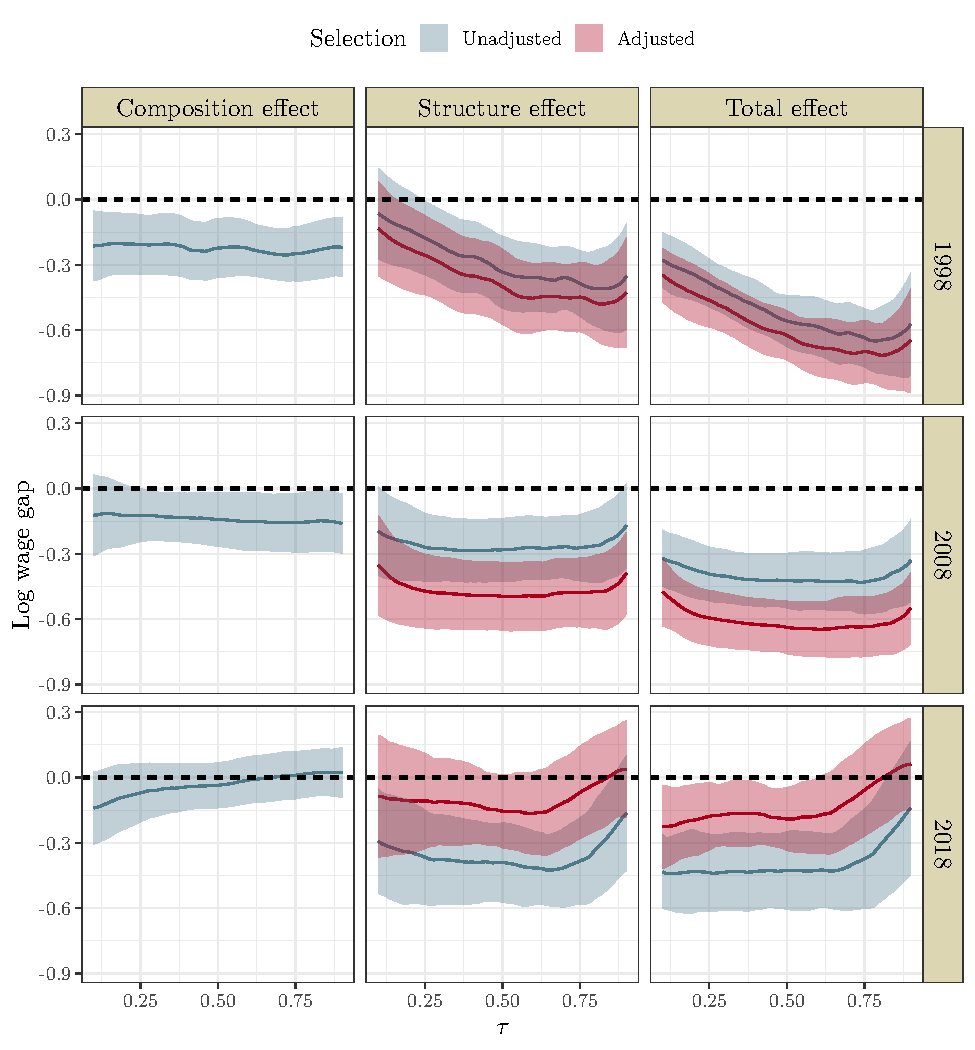
\includegraphics[width=.8\textwidth]{./figure/RuralDecom_all_all}
	\caption{Rural wage decomposition}
	\label{fig:decomMainResultRur}
\end{figure}

Rural areas saw remarkable improvements between 1998 and 2008, except for wage groups below the first quartile. In the 90th percentile, the gap declined from -0.57 to -0.33, but in the 10th percentile the gap increased from -0.28 to -0.32 (see figure \ref{fig:decomMainResultRur}). The very large gaps in higher wage groups in 1998 were due to the types of jobs that women were employed in. The majority of rural workers, especially women, held non-skilled jobs in the agricultural sector, while men dominated high-paying skilled jobs. Moreover, there was also a vast difference in CE -- approximately 40.1\% of TE at the median. With the improvement of CE and women’s increasing participation in high-paying occupations and industries, the gender wage gap shrank in the next decade among the upper wage percentiles. This shrinkage accelerated after 2008, as women increased their involvement in high-paying managerial and technical positions by almost twofold (see figures \ref{fig:industryUrbRur} and \ref{fig:occupationUrbRur}).\par

After 1998, the gap continued to increase below the median while it declined at the median and in higher wage groups. This dynamic reversed the shape of gender wage gap distribution: in 1998, low-earning women earned closer to their male counterparts, but they gradually came to lose against men, whereas high-earning women began to reach parity with men by 2018. An important reason for this worsening in the bottom groups is the types of jobs that are available in rural areas. Jobs in lower-wage percentiles are dominated by non-skilled work in the agricultural sector, which are labour-intensive physical jobs. Men are more involved in the physically demanding tasks, which are generally paid better; thus, over time -- as more labour opportunities shift their preferences to other industries, and given the lower availability of men in the agricultural sector due to widespread out-migration -- the asking price for men has increased by more than that of women, leading to wage gap divergence at the lower end.\par

In terms of CE, women in rural areas have almost reached parity with men. In 1998, median CE was -0.23 points of log wage, but this declined substantially in both decades to -0.04. By 2018, only at the lower end were women behind men in distribution of observed wage characteristics. During the same time, women in the 90th percentile pulled slightly ahead of men, from being markedly behind. In contrast, SE has changed its distributional shape over time, similar to TE. Median and lower-earning women have particularly suffered from the worsening SE, overshadowing their gains in CE. Similar to urban areas, in rural areas SE plays the dominant role in determining the overall gap.\par

\subsection{Selection adjusted decomposition}

In urban areas, after adjustment for the selection bias, the gender wage gap is further exacerbated -- more than doubling through both decades and exhibiting an even greater disparity, especially in the lower wage percentiles. In all surveys, adjusted female wage distributions are lower than unadjusted distributions, indicating positive selection -- that is, women with higher levels of observed wage-determining characteristics are employed compared to the overall female working-age population of that period. The degree of sample selection is higher in 1998, with the largest impact of adjustment occurring at the lowest wage percentiles. Over time, the adjusted total gap declined across the distribution, indicating a reduction in differences in characteristics between employed women and all working-age women. At the median, the adjusted total wage gap declined from -0.77 in 1998 to -0.63 in 2018, whereas the 90th percentile saw improvement to -0.35 from -0.42 (see table \ref{tab:adjDecom}).\par 

Compared to urban areas, rural areas exhibit more nuanced selection results. In the first two survey years, there was a positive selection of the women into the labour force, which further increased the adjusted wage gap. During these years, non-skilled work and few managerial jobs constituted the rural job market. The workforce characteristics of women were poor, and they lagged substantially behind men. Whatever few higher-wage paying jobs were available were taken by a few educated women, and the rest of the low-paying jobs were taken by women who were similar to the general rural working-age population, leading to a slight positive selection into the labour force. But, at the last survey in 2018, rural jobs bifurcated into service and non-skilled jobs. However, at this time, much of the female working-age population had taken advantage of the available educational opportunities, made accessible by recently opened community colleges.\par 

As a result, the educated female working-age pool had job opportunities in two areas: jobs in the growing service sector, and established elementary occupations. However, service-sector jobs; especially market-based service sector jobs; did not grow fast enough in rural areas to absorb this new surplus of college-educated young working women. At the same time, those employed in non-skilled occupations pulled down the average human capital of the employed. This led to a strange situation, wherein a large number of women with greater human capital were not employed and those who were employed in wage jobs had either low or insufficient human capital. Thus, our analysis finds women in rural areas to be negatively selected into the labour force, and the adjusted wage gap distribution is lower than the raw wage gap.\par 

\subsection{Household dynamics and female participation}

According to the model of home production, female household members are less likely to join the job market if their market potential is less than that of male household members. We test this hypothesis with the 2011 census, using four different logit regression models of engagement in employment -- with a key explanatory variable being the education gap, which is a proxy for the difference between market earning potentials for men and women.\par 


\begin{table}[htb]
	\caption{Female engagement in employment and gender education gap}
	\centering
	%\resizebox{\linewidth}{!}{
\begin{tabular}{lcccc}\midrule \midrule
   & Gender-wise & \multicolumn{3}{c}{Spousal pairs} \\
   \cmidrule(l{3pt}r{3pt}){2-2} \cmidrule(l{3pt}r{3pt}){3-5}		
                  & All                     & All                     & Daughter-in-law 			   & Household head\\  
   \midrule
   Panel A:& \multicolumn{4}{l}{Engaged in any work as an employee}\\
   \midrule
   Gender education gap  & -0.021$^{***}$          &   -                     &   -                     &  -\\   
                         & (0.003)                 &                         &                         &   \\   
   Spousal education gap & -                       & -0.054$^{***}$          & -0.029$^{***}$ 		   & -0.055$^{***}$\\   
                         &                         & (0.003)                 & (0.005) 				   & (0.003) \\   
   Years of schooling    & 0.071$^{***}$           & 0.053$^{***}$           & 0.087$^{***}$ 		   & 0.053$^{***}$ \\   
                         & (0.007)                 & (0.010)                 & (0.010) 				   & (0.010)\\     
   \midrule    
   Pseudo R$^2$          & 0.08099                 & 0.08142                 & 0.08941 				   & 0.08390\\ 
   \midrule   
   \midrule
   Panel B:& \multicolumn{4}{l}{Engaged in own account work}\\
   \midrule
   Gender education gap  & -0.004$^{**}$           &  -                      &  -                      & - \\   
   					  	 & (0.002)                 &                         &                         &   \\   
   Spousal education gap & -                       & 0.010$^{***}$           & 0.0001				   & 0.012$^{***}$ \\   
   						 &                         & (0.002)                 & (0.002)				   & (0.002)\\  
   Years of schooling    & -0.045$^{***}$          & -0.041$^{***}$          & -0.081$^{***}$		   & -0.032$^{***}$ \\   
   						 & (0.008)                 & (0.005)                 & (0.008)				   & (0.004) \\ 
     \midrule
   Pseudo R$^2$          & 0.18033                 & 0.22762                 & 0.23328				   & 0.22494 \\ 
   Observations          & 2,210,575               & 653,309                 & 114,547				   & 538,762 \\  
   \midrule
   \midrule
   \multicolumn{5}{p{15.2cm}}{\footnotesize{ District-wise clustered standard-errors in parentheses; Signif. Codes: ***: 0.01, **: 0.05, *: 0.1; Included control variables are age, age squared, caste groups, first component of dwelling characteristics' principal component analysis, urban dummy and districts; Spouse of household head include both wives of male household heads as well as female household heads; Source: authors' estimation.}}\\
\end{tabular}%}
\label{tab:logitGenderedEngagementsInJobs}
\end{table}


 

In the first model, we use the gender education gap -- i.e., the difference in mean years of schooling for men and women in a household -- to understand its effect on the employment of the women from that household. It is a rough measure, as it aggregates both married and unmarried household members among whom there may not be a marital relationship or gendered work division, e.g., father and teenage daughters. Nevertheless, the coefficient is negative, with both statistical and economical significance. An additional year of schooling increase for men compared to women reduces the employee status of the women by -0.02 in log odds (see table \ref{tab:logitGenderedEngagementsInJobs}). We subsequently make the measurement more precise by including all types of husband-wife pairs in column 2. The coefficient increases in magnitude to -0.05 in log odds. We further partition the dataset into two spousal pair types: (a) male head and his wife, or female head and her husband; and (b) son and daughter-in-law in a multi-generational family. In this division of spousal pair types, we find differences in both the magnitude of the spousal education gap and its importance vis-\'{a}-vis years of schooling. Among the wives of heads of households, an additional year in a spousal education gap penalises employment probability by -0.05 in log odds, which is approximately equal to gains from an additional year of schooling for the wife. However, among daughters-in-law, the effect of the spousal education gap is approximately half that of wives of heads of households and is overshadowed by the returns from years of schooling.\par

The continued increase in the magnitude of the coefficient of the education gap when moving from the first column to the third and then to the fourth column reinforces the argument that the burden on women increases when they pass from being a daughter to being a daughter-in-law and then finally to being the wife of the head of the household. The first coefficient is weighed down by the presence of daughters, who face fewer occupational barriers compared to daughters-in-laws and wives of the heads of the household. Once the daughter gets married, the hindrance of the education gap increases from -0.021 to -0.029. As a newlywed in her husband’s family, she has the support of other family members in childrearing and household chores, but she faces more stigma around entering the labour force compared to when she was unmarried. Finally, when her family moves away from her husband’s parents, she no longer enjoys that support and now must manage the home production mostly by herself. As a result, at this stage, her improvement due to additional years of schooling is completely offset by her spousal education gap.\par

We check this result against how the spousal education gap affects engagement in own-account work. Despite the statistical significance, thanks to the generous sample size, we no longer find an economically significant negative coefficient in any of the models. The sign of the spousal education gap also changes to positive, and its magnitude decreases by approximately five times. Even more interesting is that the sign of years of schooling flips to negative, meaning the more educated are less likely to be involved in own-account work. The results in panel B, in conjunction with those panel A, imply that the spousal education gap is important when women want to join the job market but is not a significant factor when they engage in own-account work. In probit specifications, the results for both panels do not change but have smaller coefficients (see annex table A7).\par

Next, we look into the time allocated to home production and find that the penalty of being a woman has hardly budged in a decade (see table \ref{tab:genderedTimeUse}). The coefficient of the matched results are similar to the baseline regressions. In 2018, unemployed women, in general, spent 102 minutes more than unemployed men doing household chores, whereas if they were employed, they did 89 more minutes of household work than unemployed men. This is in contrast to men, who hardly share the burden of home production: the figure \ref{fig:chores_III} is explicit in showing this. Whatever the employment status of women, they work 2-3 hours per day in home production, while men don’t put in even an hour of work.\par


\begin{table}[htbp]
   \caption{Gendered evaluation of time spent doing household chores}
   \centering
   %\resizebox{\linewidth}{!}{
   \begin{tabular}{lcccccc}
      \midrule \midrule
      & \multicolumn{6}{c}{Total hours spent on household chores }\\
      \cmidrule(l{3pt}r{3pt}){2-7}
      		& \multicolumn{2}{c}{NLFS II, 2008} & \multicolumn{2}{c}{NLSS III, 2011}
      		& \multicolumn{2}{c}{NLFS III, 2018} \\
      \cmidrule(l{3pt}r{3pt}){2-3} \cmidrule(l{3pt}r{3pt}){4-5} \cmidrule(l{3pt}r{3pt}){6-7}			
       Variables     & (1)            & (2)             & (3)            & (4)          & (5)            & (6)\\  
      \midrule
      Female                    & 2.37$^{***}$   & 2.43$^{***}$   & 2.47$^{***}$   & 2.59$^{***}$ & 1.71$^{***}$   & 1.70$^{***}$\\   
                                & (0.025)        & (0.039)        & (0.050)        & (0.081)      & (0.020)        & (0.028)\\   
      Employed                  & -0.497$^{***}$ & -0.474$^{***}$ & -0.135$^{***}$ & -0.143       & -0.173$^{***}$ & -0.172$^{***}$\\   
                                & (0.027)        & (0.043)        & (0.051)        & (0.093)      & (0.024)        & (0.040)\\   
      Female$\times$Employed  & -0.179$^{**}$  & -0.183$^{**}$  & -0.212$^{**}$  & -0.214$^{*}$ & -0.224$^{***}$ & -0.214$^{***}$\\   
                                & (0.070)        & (0.078)        & (0.085)        & (0.117)      & (0.054)        & (0.061)\\   
      \midrule
      
      Observations              & 41,602        & 41,602         & 15,650         & 15,650       & 44,549         & 44,549\\  
      R$^2$                     & 0.385        & 0.346        & 0.354        & 0.335      & 0.335        & 0.303\\  
      Adjusted R$^2$            & 0.385        & 0.346        & 0.353        & 0.334      & 0.335        & 0.303\\  
      \midrule \midrule
      \multicolumn{7}{p{15.2cm}}{\footnotesize{Model 1, 3 \& 5 are unmatched, whereas model 2, 4 \& 6 are matched with generalized full matching; Error bands in unmatched and matched models are HC1 robust standard errors and matched-subgroup-wise clustered standard errors respectively; Signif. Codes: ***: 0.01, **: 0.05, *: 0.1; Controls included are age, age squared, years of schooling, urban dummy, household size, caste groups, house ownership, \& land ownership;  Source: authors' estimation.}}\\
      \end{tabular}%}
  \label{tab:genderedTimeUse}
\end{table}


 

It is true that in earlier years, these male-female disparities were even larger (see annex figure A3). Nevertheless, the same results also inform us that the 40-minute decline observed for women between 2008 and 2018 has less to do with men increasing their share of burden -- on other words, substitution across gender is inelastic. Rather, this decline could have come from adoption of time-saving technologies and infrastructure development. For example, two of the tasks included in the household chores variable are time required to fetch firewood/dung (i.e., fuel) and time to fetch water. The widespread take-up of liquefied petroleum gas and electricity, which occurred in the both decades, decreased fuel-fetching time, and increased access to tapped drinking water decreased water-collecting time. Both of these, along with other time-saving changes, have led to women seeing some improvements in their time allocation to home production over the two decades studied here. But similarly-sized coefficients describing a large gap vis-\'{a}-vis men across different datasets and estimation procedures (see table \ref{tab:genderedTimeUse}) indicate that women were and are contributing disproportionately to home production.\par

\begin{figure}[htb!]
	\centering
	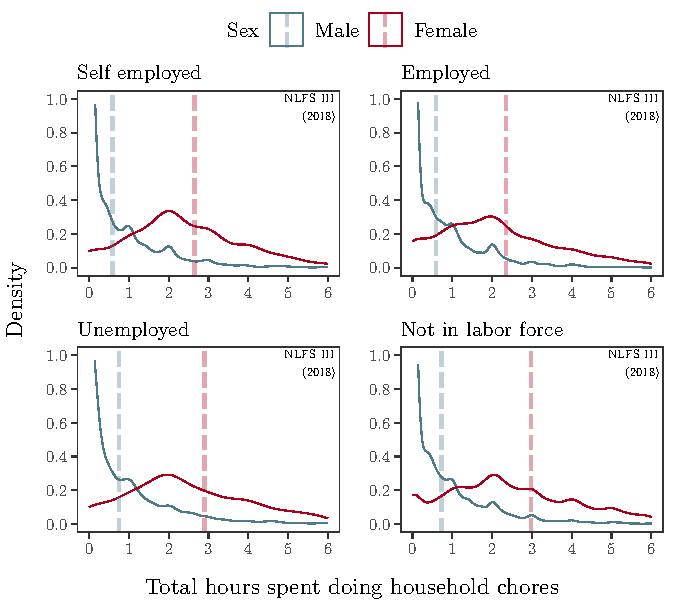
\includegraphics{./figure/chores_NLFS_III}
	\caption{Employment status and gendered time allocation on household chores in 2018. Vertical dashed lines indicate group-wise means.}
	\label{fig:chores_III}
\end{figure}

\subsection{Discussions}

Our decomposition results align with findings in the literature showing a slowdown in wage convergence, possibly due to a ‘sticky floor’ or a ‘glass ceiling’ effect. In India, a study by ~\citet{Deshpande2018} reveals a persistent, unexplained gender wage gap despite improvements in women’s wage-earning characteristics relative to men. Like our findings, they identify a sticky floor effect, with a growing structural impact particularly among low-wage earners. Another study by ~\citet{Yamamoto2019} using a different Nepalese data reports a substantial wage gap and a strong structural effect. However, these studies do not fully consider factors like the nature of work, specific work-related experience, and fine-grained workplace attributes. Similarly, we also face limitations in accounting for these variables, due to methodological and data constraints.\par

While worker characteristics significantly impact wage gaps, workplace attributes are also crucial.~\citet{Chatterji2011} find that only a small fraction of the gender earnings gap in Great Britain can be attributed to employee characteristics, emphasizing the substantial role of workplace attributes there. Newer datasets with more work diversity and pay variations will have higher structure effects when decomposed without sufficient work-related details. So, some of our increasing structural effect stems from not including work specifics in the wage equation. Despite this limitation, human capital specifications have quite strong explanatory power. For instance, in~\citet{Blau2017}, human capital specifications account for 82.1\% of the female-to-male log wage ratio, which increases to 91.6\% when industry and occupation variables are added. Thus, even when only looking at the human capital specifications, we can find change in their relative importance for the wage gap. In our results for rural area, there is a substantial convergence in composition effect between 1998 and 2008, which points out that Nepal has utilized a powerful source of convergence to a full effect in these two decades.\par

In their consideration of selection, ~\citet{Maasoumi2019} reach different conclusions than without. We also find that the positive selection of highly-educated women into the labour force obscures the true gender wage gap, especially in urban areas. Additionally, differential outcomes in different wage groups -- i.e., stagnation below median wages but convergence above it -- emphasise the need for more literature on distributional decomposition that accounts for selection. It should be noted that selection outcomes can vary depending on the applied method:~\citet{Machado2017} draws different conclusions from the same data by using different methods. Despite this variability, selection remains a critical issue, as~\citet{Heckman1974} and~\citet{Gronau1974} have noted, as it provides a ‘truer’ depiction of the labour market than models without it.\par

Increasing SE, and the weakening role of gender parity in human capital in improving the gap, means that we have to look at structural factors affecting women's meaningful labour market outcomes. One such important determinant is intra-spousal negotiation.~\citet{Bertrand2015} report a societal aversion to a wife earning more than her husband. These societal attitudes affect marriage formation and wives’ labour force participation, income, marriage satisfaction, and household chores. For example, in developed countries, highly-skilled women tend to marry less often than their less-skilled counterparts~\citep{Bertrand2020social}, and the marriage gap depends on societal attitudes toward working women. Similarly, in Nepal, spousal negotiation looks unfavorable for women. Our results show that a greater spousal education gap makes it difficult for women to participate in the labour market as an employee. The gap’s effect increases with the increase in a woman’s household stature, from daughter-in-law to wife of the head of the household. This way of sorting women to home production aligns with the prediction of the stylized home production model of~\citet{Cortes2020}.\par

In addition to the gendered sorting into employment, the time devoted to home production is also very gendered. We find that men avoid contributing even when they are not employed, and this pattern has not changed in the two decades under study. As a result women who want to be employed currently face the ``dual burden'' of work and home production: if they are employed, they have to do hours at their job, but they also have to put in hours at home as if they were not employed -- the difference of being employed was a mere 12.8 minutes in 2018. This dual burden is the norm among women in the labour market almost everywhere~\citep{Hochschild2012}.\par

A similar result is reported in southern Europe by~\citet{Lichard2021}. In a more specific setting,~\citet{Alvarez2019} study differential allocation of time on nonworking days in dual-earner couples. They find that on their nonworking days, wives take on most of the household tasks. These skewed home-production responsibilities amplify the wage gap. For example, in Europe, while mothers face motherhood penalties after the birth of a child, fathers enjoyed wage premiums~\citep{CukrowskaTorzewska2020}. Similarly,~\citet{Cortes2020} report that two-thirds of the remaining gender earnings gap in the US is due to childrearing responsibilities, which are imposed solely on women. These types of barriers can come in different forms; for instance, in Italy, the social norm of marriage within the community preserves social norms against women working, which discouraged women from participating in jobs, eventually increasing the gender workforce participation gap~\citep{Righetto2023}. As a consequence of non-participation in home production, men can often work inflexible jobs for longer hours, take fewer leaves, and be in jobs that demand on-call availability, which provides structural advantages. Employers often reward these advantages, increasing men’s earning potential in the labour market~\citep{Goldin2014}.\par

Recently, the role of psychological factors keeping women out of labour market participation have begun to be recognised. In the case of high-wage US workers,~\citet{Francis2023} find that gender-based pay gaps persist due to career interruptions and differences in risk preferences, particularly at the executive level. Even among recent graduates, preferences might lead women to make very different choices. For example,~\citet{Piazzalunga2018}'s study of recent graduates finds that childcare, part-time employment availability, and traditional gender norms were important in determining the gender wage gap.\par